\documentclass[Arkitektur/System_main.tex]{subfiles}
\begin{document}
\subsubsection{PlayerSideApp} \label{sec:playersideapp_application_model}
Der er til PlayerSideApp, som skal køre på 'PSoC Player side', som er en del af 'Player side' blokken, udviklet en applikationsmodel. På PSoC'en afvikles C kode, og det er derfor ikke direkte muligt at benytte klasser, men der laves stadig et klassediagram som en del af applikationsmodellen (se figur \ref{fig:CD_PlayerSide}. Klasserne implementeres som forskellige moduler (separate header og implementeringsfiler).

\begin{figure}[H]
    \centering
    \centering
    \makebox[\textwidth][c]{%
        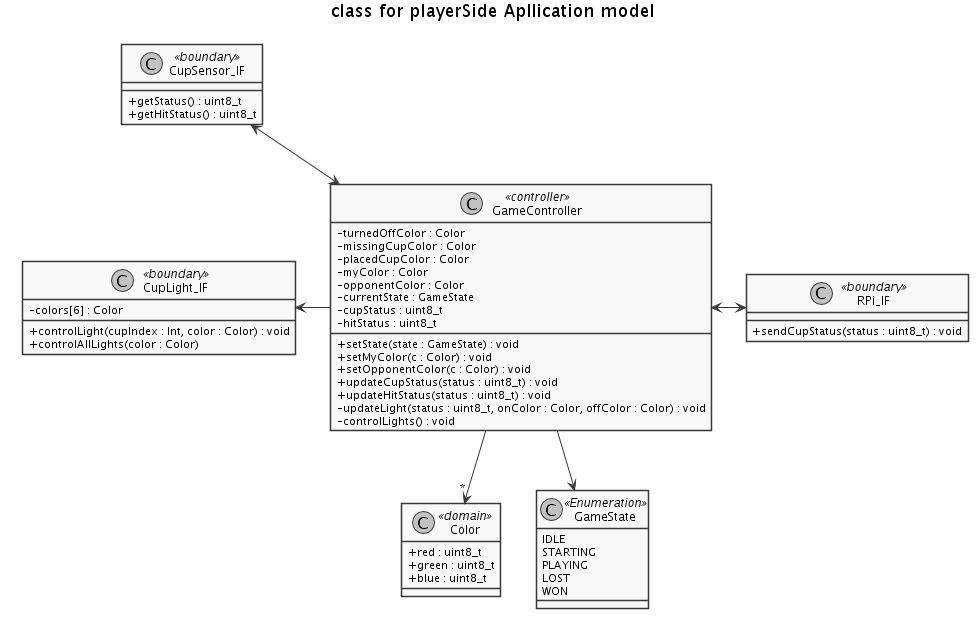
\includegraphics[width=1.2\textwidth]{Arkitektur/Softwarearkitektur/Applikationsmodel/PlayerSide/graphics/classDiagram.png}
    }
    \caption{Klassediagram for playerSideApp}
    \label{fig:CD_PlayerSide}
\end{figure}


{\large\textbf{Tilstandsmaskine for playerSideApp}}\\
Programmet bygges op omkring en tilstandsmaksine, se figur \ref{fig:playerSide_SM}. Dette er den vigtigste del af denne applikationsmodel. Denne tilstandsmaskine er med udgangspunkt i GameController klassen. hvis der kaldes en metode i en anden klasse noteres dette med '.' operatoren. De steder hvor der ikke benyttes '.' operatoren er der tale om en metode i GameController klassen. Tilstandene styres af RPi vha. metoden setState(). Det fremgår af figuren at tilstandsmaskinen kun kan skifte til fx tilstanden LOST hvis den er i tilstanden PLAYING. Dette er ikke sandt. Tilstandsmaskinen kan skifte til hvilket som helst tilstand bestemt af parameteren til setState() metoden. Alle disse tilstandsændringer er ikke medtaget i diagrammet for overskuelighedens skyld. Det som ses på diagrammet, er de ændringer der vil ske under normale omstændigheder. Afhængig af hvilken tilstand applikationen er i, skal der udføres forskellige ting. Der er de fem tilstande: IDLE, STARTING, PLAYING, LOST og WON. IDLE er tilstanden hvor der ikke er nogen der bruger systemet. Her skal der slukkes for alt lys. Dette gøres ved \textbf{entry} for tilstanden. LOST og WON er tilstandene hvor der er fundet en vinder, og den givne side har enten vundet eller tabt. I disse tilstande skal alle kopper lyse med en farve. Når man vinder skal alle kopper lyse med sin farve (myColor), og når man taber skal de lyse med modstanderholdets farve (opponentColor). Dette udføres ved \textbf{entry} for tilstandene. STARTING er tilstanden hvor spillet opsættes (svare til UC1). Ved tilstanden STARTING skal lyset under hver kop være styret af om der er en kop eller ej. Hvis der er en kop skal den lyse med en farve (placedCupColor) og hvis der ikke er en kop skal den lyse med en anden (missingCupColor). Dette udføres til dels ved \textbf{do} for tilstanden. Her kaldes metoden Controller(), som skal sørge for styre lyset. Derudover skal cupStatus opdateres, dette gøres i \textbf{entry} og hver gang der fjernes eller tilføjes en kop (se figur \ref{fig:playerSide_STARTING_SD}). Der sendes information om hvilke kopper der er placeret på bordet (status) til RPi når der sker en ændring (se figur \ref{fig:playerSide_STARTING_SD}), men det sendes også ved \textbf{entry}.
PLAYING er tilstande hvor spillet er i gang (svare til UC2). I tilstanden PLAYING skal der stort set ske det samme som i tilstanden STARTING, det er bare nogle andre farver der skal bruges. Derudover skal der nu også håndteres at en bold rammer i en kop. Dette ses i \ref{fig:playerSide_PLAYING_SD}.

Funktionen Controller kaldes hele tiden i hvert tilstand. Den har til opgave at styre lyset på baggrund af det data som den har modtages fra CupSensor\_IF klassen. Den skal også kalde metoden RPI\_IF\_handleData i RPi\_IF klassen, dette er for RPi\_IF får mulighed for at tjekke om der er modtaget nyt data, og herefter kalde de nødvendige metoder hvis dette er tilfældet. Controller funktionen skal også starte/stoppe en timer som skal bruges til at blinke med lyset når en bold rammer i. Denne timer kalder funktionen interruptBlink hvergang lyset skal skifte tilstand. 

\begin{figure}[H]
    \centering
    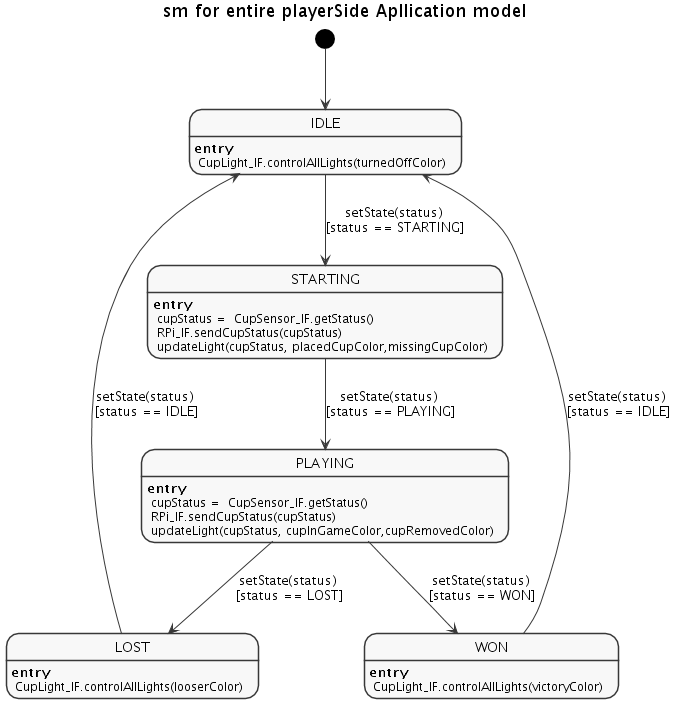
\includegraphics[width=\textwidth]{Arkitektur/Softwarearkitektur/Applikationsmodel/PlayerSide/graphics/state.png}
    \caption{Tilstandmaskine for playerSideApp}
    \label{fig:playerSide_SM}
\end{figure}


{\large\textbf{Controller:  GameController}}\\
GameController er den centrale klasse for alle use cases. Den sørger for at sende og modtage data gennem klassen RPi\_IF. Alt modtaget data bliver evalueret i GameController og sendt videre i overensstemmelse med protokollen og use case flow. Klassen varetager alt logikken og de flest beslutninger for player side. 

{\large\textbf{Attributbeskrivelser: GameController}}
\begin{adjustwidth}{1cm}{0pt}
\textbf{turnedOffColor:} Dette er den farve som CupLights skal have når currentState er IDLE. \\[0.2cm]
\textbf{missingCupColor:} Dette er den farve som en CupLight skal have når der IKKE er en kop imens currentState er STARTING. \\[0.2cm]
\textbf{placedCupColor:} Dette er den farve som en CupLight skal have når der er en kop imens currentState er STARTING. \\[0.2cm]
\textbf{myColor:} Dette er farven på det hold som har deres kopper på den Player side som PSoC'en er en del af.\\[0.2cm]
\textbf{opponentColor:} Dette er farven på det hold som har deres kopper på den MODSATTE Player side end den som PSoC'en er en del af.\\[0.2cm]
\textbf{currentState:} Dette er systemets nuværende tilstand.\\[0.2cm]
\textbf{cupStatus:} Denne attribut repræsentere hvilke kopholdere, hvor en kopholder er placeret på den. De 6 mindst betydende bits repræsenterer, om der er en kop eller ej. Hvis et bit er 1 betyder det at der er en kop. Koppernes placering på bordet og deres bit nummer er map'et på samme måde, som beskrevet i protokollen. \\[0.2cm] 
\textbf{hitStatus:} Denne attribut repræsentere hvilke kopholdere, som indeholder en kop hvor en bold er ramt i. De 6 mindst betydende bits repræsenterer om en bold er ramt i en kop eller ej. 1 betyder at der er ramt en bold i koppen. Koppernes placering på bordet og deres bit nummer er map'et på samme måde som beskrevet i protokollen. \\[0.2cm]

\end{adjustwidth}


    {\large\textbf{Funktionsbeskrivelser: GameController}}\\[0.2cm]
    \textbf{setState(state: GameState) : void}
    \begin{adjustwidth}{1cm}{0pt}
    \textbf{Beskrivelse:} Skal sørge for at ændre tilstanden i tilstandsmaskinen. Dette gøres ved at indstille currentState. Skal også sørge for at udføre de ting som er specificeret i \textbf{entry} i tilstandsmaskinen. \\[0.2cm]
    \textbf{Parametre:} state : GameState: tilstanden som der skal skiftes til. \\[0.2cm]
    \textbf{Retur værdi:} ingen \\[0.2cm]
    \textbf{Bivirkninger:} ingen \\[0.2cm]
    \end{adjustwidth}
    
    \textbf{setMyColor(c: Color) : void}
    \begin{adjustwidth}{1cm}{0pt}
    \textbf{Beskrivelse:} Skal indstille myColor. \\[0.2cm]
    \textbf{Parametre:} c: Color: Den farve som myColor skal indstilles til. \\[0.2cm]
    \textbf{Retur værdi:} ingen \\[0.2cm]
    \textbf{Bivirkninger:} ingen \\[0.2cm]
    \end{adjustwidth}
    
    \textbf{setOpponentColor(c: Color) : void}
    \begin{adjustwidth}{1cm}{0pt}
    \textbf{Beskrivelse:} Skal indstille opponentColor \\[0.2cm]
    \textbf{Parametre:} c: Color: Den farve som opponentColor skal indstilles til.\\[0.2cm]
    \textbf{Retur værdi:} ingen\\[0.2cm]
    \textbf{Bivirkninger:} ingen\\[0.2cm]
    \end{adjustwidth}
    
    \textbf{updateCupStatus(status: uint8\_t) : void}
    \begin{adjustwidth}{1cm}{0pt}
    \textbf{Beskrivelse:} Skal sørge for at håndtere alt logikken, der skal ske når der fjernes eller tilføjes en kop. Den skal bl.a. indstille cupStatus attributen, og sende den nye cupStatus videre til RPi, vha. RPi\_IF.\\[0.2cm]
    \textbf{Parametre:} status: uint8\_t: den værdi cupStatus skal indstilles til. Har samme format som cupStatus.\\[0.2cm]
    \textbf{Retur værdi:} ingen\\[0.2cm]
    \textbf{Bivirkninger:} ingen\\[0.2cm]
    \end{adjustwidth}
    
    \textbf{updateHitStatus(status: uint8\_t) : void}
    \begin{adjustwidth}{1cm}{0pt}
    \textbf{Beskrivelse:} Skal sørge for at håndtere alt logikken der skal ske når en bold rammer i en kop. Den skal bl.a. indstille hitStatus attributen.\\[0.2cm]
    \textbf{Parametre:} status: uint8\_t: den værdi hitStatus skal indstilles til. Har samme format som hitStatus.\\[0.2cm]
    \textbf{Retur værdi:} ingen\\[0.2cm]
    \textbf{Bivirkninger:} ingen\\[0.2cm]
    \end{adjustwidth}



\textbf{controlLights() : void}
\begin{adjustwidth}{1cm}{0pt}
\textbf{Beskrivelse:} Hjælpefunktion som bruges til at styre de forskellige CupLights. Den skal afhængig af currentState og CupStatus styre lyset. Hvis currentState er STARTING skal hver CupLight styres til at lyse med enten missingCupColor eller placedCupColor afhængig af cupStatus. Hvis currentState er PLAYING, skal hver CupLight styres til at lyse med enten myColor eller opponentColor afhængig af cupStatus.  \\[0.2cm]
\textbf{Parametre:} ingen\\[0.2cm]
\textbf{Retur værdi:} ingen\\[0.2cm]
\textbf{Bivirkninger:} ingen\\[0.2cm]
\end{adjustwidth}

\textbf{Controller() : void}
\begin{adjustwidth}{1cm}{0pt}
\textbf{Beskrivelse:}Det første der gøres er at kalde RPI\_IF\_handledata fra RPI\_IF. Udover dette vil denne funktion eksekveres i de tilfælde currentState er STARTING eller PLAYING. Når systemet er i en af disse tilstande, så vil en ændring i CupStatus ændrer tilstanden af lysene ved at kalde controlLights med CupStatus. Hvis systemet er i PLAYING, så vil blinke funktionen også kontrolleres her. Er systemet ikke i nogle af disse tilstande vil blink stoppes.
\\[0.2cm]
\textbf{Parametre:} ingen\\[0.2cm]
\textbf{Retur værdi:} ingen\\[0.2cm]
\textbf{Bivirkninger:} ingen\\[0.2cm]
\end{adjustwidth}

\textbf{interruptBlink() : void}
\begin{adjustwidth}{1cm}{0pt}
\textbf{Beskrivelse:} Denne funktion bliver kaldt hver gang en timer overflower. Funktionen skal toggle farven for de kopper som er blevet ramt. Til dette skal attributten hitStatus benyttes. De to farver der skal toggles imellem er myColor og opponentColor.
\\[0.2cm]
\textbf{Parametre:} ingen\\[0.2cm]
\textbf{Retur værdi:} ingen\\[0.2cm]
\textbf{Bivirkninger:} ingen\\[0.2cm]
\end{adjustwidth}

{\large\textbf{Boundary:  RPi\_IF}}\\
Klassen skal modtage kommandoer fra Raspberry pi, og sende data til raspberry pi. Der modtages hovedsageligt data om hvilken tilstand systemet er i og der sendes hovedsageligt koppernes status (om de er der eller ej)

{\large\textbf{Funktionsbeskrivelser: RPi\_IF}}\\[0.2cm]
\textbf{sendCupStatus(status: uint8\_t) : void}
\begin{adjustwidth}{1cm}{0pt}
\textbf{Beskrivelse:} Skal sørge for at sende den nødvendige data som specificeret i protokollen vha. I2C, for at sende den cupStatus som er specificeret i parameteren status .\\[0.2cm]
\textbf{Parametre:} status: uint8\_t: Den status som skal sendes videre til RPi \\[0.2cm]
\textbf{Retur værdi:} ingen \\[0.2cm]
\textbf{Bivirkninger:} ingen \\[0.2cm]
\end{adjustwidth}

\textbf{RPI\_IF\_handledata() : void}
\begin{adjustwidth}{1cm}{0pt}
\textbf{Beskrivelse:}
Denne metode skal sørge for modtagelsen af beskeder sendt over I2C til PSoC Player side. Den skal bruge funktionerne setState, setMyColor og setOpponentColor i GameController klassen alt efter om en besked omkring farveændring eller ændring af state  modtages fra RPI'en.
\\[0.2cm]
\textbf{Parametre:} ingen \\[0.2cm]
\textbf{Retur værdi:} ingen \\[0.2cm]
\textbf{Bivirkninger:} ingen \\[0.2cm]
\end{adjustwidth}

{\large\textbf{Boundary:  CupLight\_IF}}\\
Klasse som skal styre lyset under hver kop.

{\large\textbf{Attributbeskrivelser: CupLight\_IF}}
\begin{adjustwidth}{1cm}{0pt}
\textbf{colors[6]: Color } Et array med der indeholder hver kops farve. Dette ændres løbende. \\[0.2cm]
\end{adjustwidth}
{\large\textbf{Funktionsbeskrivelser: CupLight\_IF}}\\[0.2cm]
\textbf{controlLight(cupIndex: Int, color : Color) : void}
\begin{adjustwidth}{1cm}{0pt}
\textbf{Beskrivelse:} Skal indstille farven på den CupLight med index'et cupIndex til farven color. \\[0.2cm]
\textbf{Parametre:}  cupIndex: Int: Den CupLight hvis lys skal styres. Dette index har samme nummerering som det bit numrene som er specificeret i protokollen\\color: Color: Den farve som den givne CupLight skal have \\[0.2cm]
\textbf{Retur værdi:} ingen \\[0.2cm]
\textbf{Bivirkninger:} ingen \\[0.2cm]
\end{adjustwidth}
\textbf{controlAllLights(color : Color) : void}
\begin{adjustwidth}{1cm}{0pt}
\textbf{Beskrivelse:} Skal indstille farven på alle CupLights farven color.
\textbf{Parametre:} color: Color: Den farve som alle CupLights skal indstilles til \\[0.2cm]
\textbf{Retur værdi:} ingen \\[0.2cm]
\textbf{Bivirkninger:} ingen \\[0.2cm]
\end{adjustwidth}


{\large\textbf{Boundary:  CupSensor\_IF}}\\
Klasse som skal håndtere signal fra Cup sensorerne. Skal informere GameController klassen når der sker en ændring på status på en af kopperne.

{\large\textbf{Funktionsbeskrivelser: CupSensor\_IF}}\\[0.2cm]
\textbf{getStatus() : uint8\_t}
\begin{adjustwidth}{1cm}{0pt}
\textbf{Beskrivelse:} Skal returnere den nuværende cup status. Cup status er hvilke kopholdere der indeholder en kop.
\textbf{Parametre:} ingen \\[0.2cm]
\textbf{Retur værdi:} uint8\_t: den nuværende cup status. Samme format som cupStatus attributten i GameController \\[0.2cm]
\textbf{Bivirkninger:} ingen \\[0.2cm]
\end{adjustwidth}

\textbf{getHitStatus() : uint8\_t}
\begin{adjustwidth}{1cm}{0pt}
\textbf{Beskrivelse:} Skal returnere den nuværende hit status. Hit status er hvilke kopper der er blevet ramt af en bold.
\textbf{Parametre:} ingen \\[0.2cm]
\textbf{Retur værdi:} uint8\_t: den nuværende hit status. Samme format som hitStatus attributten i GameController \\[0.2cm]
\textbf{Bivirkninger:} ingen \\[0.2cm]
\end{adjustwidth}


{\large\textbf{Domain:  Color}}\\
Klasse som bruges til at lagre oplysninger om de forskellige farver der skal bruges.  

{\large\textbf{Attributbeskrivelser: Color}}
\begin{adjustwidth}{1cm}{0pt}
\textbf{red:} beskriver lysstyrken af det røde lys i farven i intervallet 0-255. 0 betyder slukket og 255 betyder fuld lysstyrke \\[0.2cm]
\textbf{green:} beskriver lysstyrken af det grønne lys i farven i intervallet 0-255. 0 betyder slukket og 255 betyder fuld lysstyrke \\[0.2cm]
\textbf{blue:} beskriver lysstyrken af det blå lys i farven i intervallet 0-255. 0 betyder slukket og 255 betyder fuld lysstyrke \\[0.2cm]
\end{adjustwidth}

{\large\textbf{Enumeration:  GameState}}\\
Denne "klasse" er ikke en rigtig klasse. Den bruges til at definere de forskellige tilstande i applicationen. 

{\large\textbf{Sekvensdiagram for STARTING}}\\
Der laves sekvensdiagrammer for tilstandene STARTING og PLAYING. Der laves ikke sekvensdiagrammer for de andre tilstande, da der ikke skal ske noget i selve tilstanden, der skal kun ske noget ved \textbf{entry}, og dette er allerede beskrevet i tilstandsmaskinen. Sekvensdiagrammet for STARTING kan ses på figur \ref{fig:playerSide_STARTING_SD}

\begin{figure}[H]
    \centering
    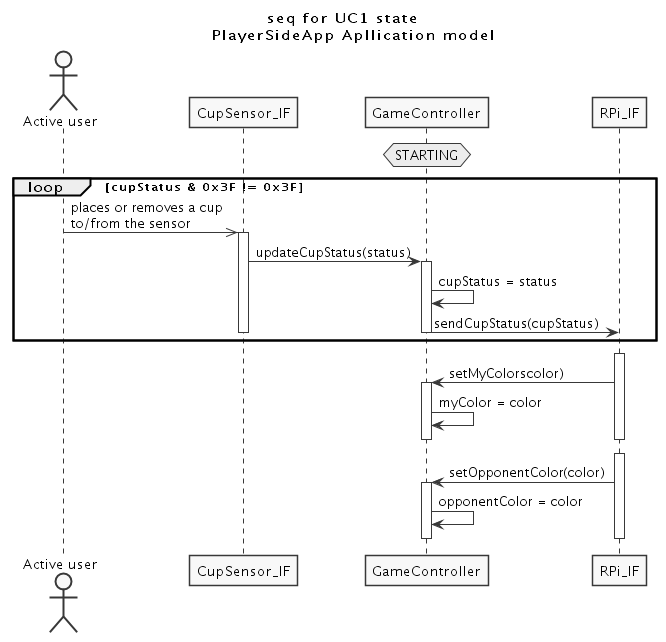
\includegraphics[width=\textwidth]{Arkitektur/Softwarearkitektur/Applikationsmodel/PlayerSide/graphics/UC1_sequence.png}
    \caption{Sekvensdiagram for tilstand STARTING}
    \label{fig:playerSide_STARTING_SD}
\end{figure}
Der er på diagrammet tegnet en aktør 'Opponent' for at vise hvornår der bliver fjernet/tilføjet en kop. Denne aktør skal (som altid) forstås som det hold som ikke har turen 'Opponent'. Når et hold skal fjerne en kop fra deres Player side er de altså 'Opponent' 
Hver gang der tilføjes eller fjernes en kop fra bordet skal denne nye status sendes til GameController og den sørger for at opdatere cupStatus attributten sende status til RPi. Lyset styres indirekte idet der i \textbf{do} delen af tilstanden kaldes controlLights() metoden som reagere på den opdaterede cupStatus og dermed styrer lyset. Når alle kopper er placeret reagere RPi'en på dette og den får information fra hjemmesiden om hvilke holdfarver der er. Når den har fået disse holdfarver sender den dem videre til PSoC'en og dette reagere RPi\_IF på og kalder de to metoderne setMyColor() og setOpponentColor()

{\large\textbf{Sekvensdiagram for PLAYING}}\\
Sekvensdiagrammet for PLAYING kan ses på figur \ref{fig:playerSide_PLAYING_SD}

\begin{figure}[H]
    \centering
    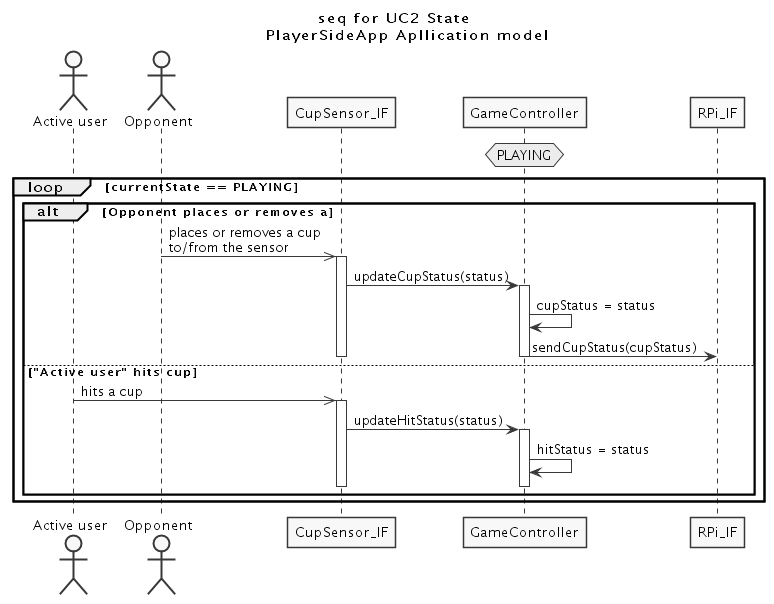
\includegraphics[width=\textwidth]{Arkitektur/Softwarearkitektur/Applikationsmodel/PlayerSide/graphics/UC2_sequence.png}
    \caption{Sekvensdiagram for tilstand PLAYING}
    \label{fig:playerSide_PLAYING_SD}
\end{figure}
Den første del af dette diagram er stort set identisk med det for tilstanden STARTING (figur \ref{fig:playerSide_PLAYING_SD}) men der skal ikke kun reageres på at en kop tilføjes eller fjernes men også om en bold rammer i en kop. Når dette sker skal hitStatus attributten opdateres. Igen styres lyset indirekte idet der i \textbf{do} delen af tilstanden kaldes controlLights() som reagere på at både hitStatus og cupStatus ændres.


\end{document}